\documentclass{standalone}
\usepackage{tikz}
\usetikzlibrary{patterns}
\usetikzlibrary{positioning}
\usetikzlibrary{patterns, positioning}
\usetikzlibrary{shapes.misc}
\usepackage[outline]{contour}
\contourlength{1.5pt} 
\usepackage[sfdefault]{ClearSans}

\begin{document}
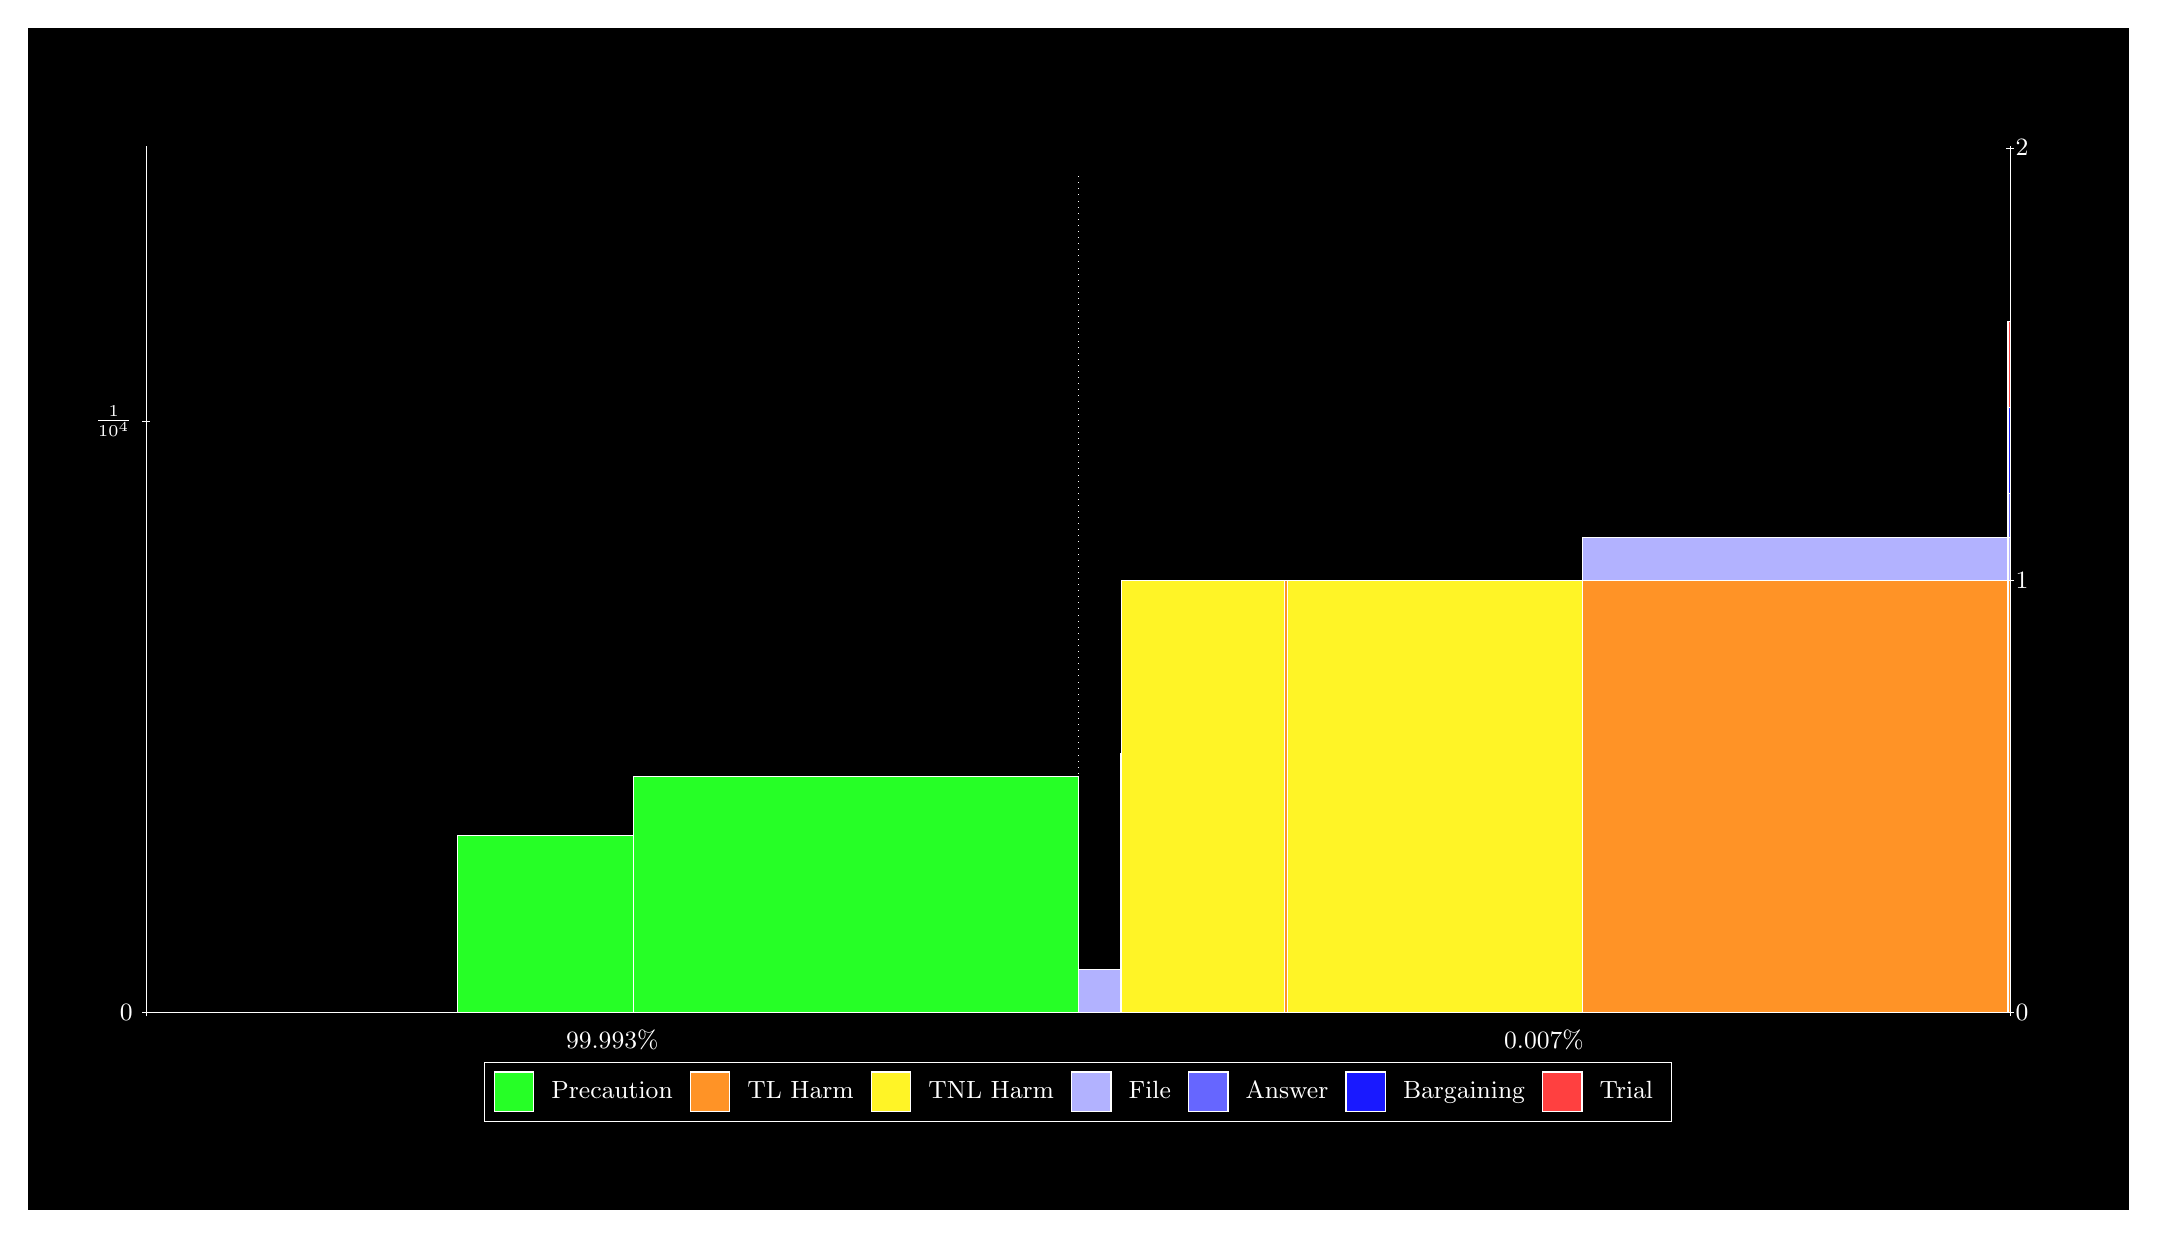
\begin{tikzpicture}
\draw[fill=black] (0,0) rectangle (26.667,15);
\draw[fill=green!85,draw=white,very thin] (5.4443,2.5) rectangle (7.685,4.7528);
\draw[fill=green!85,draw=white,very thin] (7.685,2.5) rectangle (13.333,5.5038);
\draw[fill=blue!30,draw=white,very thin] (13.333,2.5) rectangle (13.873,3.049);
\draw[fill=green!85,draw=white,very thin] (13.873,2.5) rectangle (13.879,2.5002);
\draw[fill=blue!30,draw=white,very thin] (13.873,2.5002) rectangle (13.879,3.0492);
\draw[fill=blue!60,draw=white,very thin] (13.873,3.0492) rectangle (13.879,3.5981);
\draw[fill=blue!90,draw=white,very thin] (13.873,3.5981) rectangle (13.879,4.6961);
\draw[fill=red!75,draw=white,very thin] (13.873,4.6961) rectangle (13.879,5.7941);
\draw[fill=green!85,draw=white,very thin] (13.879,2.5) rectangle (15.954,2.5002);
\draw[fill=yellow!85,draw=white,very thin] (13.879,2.5002) rectangle (15.954,7.9901);
\draw[fill=green!85,draw=white,very thin] (15.954,2.5) rectangle (15.991,2.5002);
\draw[fill=orange!85,draw=white,very thin] (15.954,2.5002) rectangle (15.991,7.9901);
\draw[fill=green!85,draw=white,very thin] (15.991,2.5) rectangle (19.737,2.5002);
\draw[fill=yellow!85,draw=white,very thin] (15.991,2.5002) rectangle (19.737,7.9901);
\draw[fill=orange!85,draw=white,very thin] (19.737,2.5) rectangle (25.133,7.9899);
\draw[fill=blue!30,draw=white,very thin] (19.737,7.9899) rectangle (25.133,8.5389);
\draw[fill=green!85,draw=white,very thin] (25.133,2.5) rectangle (25.151,2.5002);
\draw[fill=yellow!85,draw=white,very thin] (25.133,2.5002) rectangle (25.151,7.9901);
\draw[fill=blue!30,draw=white,very thin] (25.133,7.9901) rectangle (25.151,8.5391);
\draw[fill=blue!60,draw=white,very thin] (25.133,8.5391) rectangle (25.151,9.0881);
\draw[fill=blue!90,draw=white,very thin] (25.133,9.0881) rectangle (25.151,10.186);
\draw[fill=red!75,draw=white,very thin] (25.133,10.186) rectangle (25.151,11.284);
\draw[fill=green!85,draw=white,very thin] (25.151,2.5) rectangle (25.167,2.5002);
\draw[fill=orange!85,draw=white,very thin] (25.151,2.5002) rectangle (25.167,7.9901);
\draw[fill=blue!30,draw=white,very thin] (25.151,7.9901) rectangle (25.167,8.5391);
\draw[fill=blue!60,draw=white,very thin] (25.151,8.5391) rectangle (25.167,9.0881);
\draw[fill=blue!90,draw=white,very thin] (25.151,9.0881) rectangle (25.167,10.186);
\draw[fill=red!75,draw=white,very thin] (25.151,10.186) rectangle (25.167,11.284);
\draw[white,very thin] (1.5,2.5) -- (1.5,13.5);
\draw[white,very thin] (1.45,2.5) -- (1.55,2.5);
\node[font=\small,text=white, anchor=east] at (1.45, 2.5) {0};
\draw[white,very thin] (1.45,10.009) -- (1.55,10.009);
\node[font=\small,text=white, anchor=east] at (1.45, 10.009) {$\frac{1}{10^{4}}$};

\draw[white,dotted,very thin] (13.333,2.83) -- (13.333,13.17);
\draw[white,very thin] (25.167,2.5) -- (25.167,13.5);
\draw[white,very thin] (25.117,2.5) -- (25.217,2.5);
\node[font=\small,text=white, anchor=west] at (25.117, 2.5) {0};
\draw[white,very thin] (25.117,7.9899) -- (25.217,7.9899);
\node[font=\small,text=white, anchor=west] at (25.117, 7.9899) {1};
\draw[white,very thin] (25.117,13.48) -- (25.217,13.48);
\node[font=\small,text=white, anchor=west] at (25.117, 13.48) {2};

\draw[white,very thin] (1.5,2.5) -- (25.167,2.5);
\draw[white,very thin] (1.5,2.45) -- (1.5,2.55);
\node[font=\small,text=white, anchor=north] at (1.5, 2.45) {};
\draw[white,very thin] (25.167,2.45) -- (25.167,2.55);
\node[font=\small,text=white, anchor=north] at (25.167, 2.45) {};

\node[font=\small,text=white,anchor=south] at (7.4167, 1.9) {99.993\%};
\node[font=\small,text=white,anchor=south] at (19.25, 1.9) {0.007\%};
\draw (13.3333,2.5) node (B) {};
\begin{scope}[align=center]
\matrix[scale=0.5,draw=white,below=0.5cm of B,nodes={draw},column sep=0.1cm]{
\node[rectangle,draw,minimum width=0.5cm,minimum height=0.5cm,fill=green!85]{}; & \node[draw=none,font=\small,text=white]{Precaution}; &
\node[rectangle,draw,minimum width=0.5cm,minimum height=0.5cm,fill=orange!85]{}; & \node[draw=none,font=\small,text=white]{TL Harm}; &
\node[rectangle,draw,minimum width=0.5cm,minimum height=0.5cm,fill=yellow!85]{}; & \node[draw=none,font=\small,text=white]{TNL Harm}; &
\node[rectangle,draw,minimum width=0.5cm,minimum height=0.5cm,fill=blue!30]{}; & \node[draw=none,font=\small,text=white]{File}; &
\node[rectangle,draw,minimum width=0.5cm,minimum height=0.5cm,fill=blue!60]{}; & \node[draw=none,font=\small,text=white]{Answer}; &
\node[rectangle,draw,minimum width=0.5cm,minimum height=0.5cm,fill=blue!90]{}; & \node[draw=none,font=\small,text=white]{Bargaining}; &
\node[rectangle,draw,minimum width=0.5cm,minimum height=0.5cm,fill=red!75]{}; & \node[draw=none,font=\small,text=white]{Trial}; \\\\
};\end{scope}

\end{tikzpicture}
\end{document}